% system model slides

\section*{}
\subsection*{Three-Body Problem}  
\begin{frame} %-----------------------------%
\frametitle{Planar Circular Restricted Three-Body Problem}
	\begin{columns}[T]
	\begin{column}{0.5\textwidth}
  		\begin{itemize}
  			\item Motion of spacecraft \( P\) under the mutual gravitational attraction of two primaries \( m_1 \) and \( m_2 \)
			\item Nondimensionalization of the system
			\begin{itemize}
				\item \(G = 1\)
				\item Orbital period \( = 2\pi\)
				\item Single parameter to describe dynamics
			\end{itemize}	
					
 		\end{itemize}
 	\begin{equation*}
		\mu = \frac{m_2}{m_1+m_2}
		\label{eq:mass_param}
	\end{equation*}
	\end{column}
	\begin{column}[T]{0.5\textwidth}
		\begin{itemize}
			\item  \(x\) axis aligned along primaries
			\item Allows for greater structure in the dynamics
		\begin{figure}[htbp]%
        	\includegraphics[width=\textwidth]{rot_frame}%
		\end{figure}%
		\end{itemize}
	\end{column}
	\end{columns}
\end{frame}   %-----------------------------%

\begin{frame} %-----------------------------%
\frametitle{Planar Circular Restricted Three-Body Problem}
\begin{columns}
\begin{column}{0.5\textwidth}
   \begin{itemize}
   		\item Distances to each primary
		\begin{align*}
			r_1 &= \sqrt{\left( x+ \mu\right)^2 + y^2} \\
			r_2 &= \sqrt{\left( x - 1 + \mu\right)^2 + y^2}
		\end{align*}
   \end{itemize}
   \includegraphics[width = \columnwidth]{rot_frame_def}
\end{column}
\begin{column}{0.5\textwidth}
	\begin{itemize}
		\item Effective gravitational potential
	\begin{equation*}
		U = \frac{1}{2} \left( x^2 + y^2\right) + \frac{1-\mu}{r_1} + \frac{\mu}{r_2}
		\label{eq:eff_pot}
	\end{equation*}
		\item Planar Spacecraft Dynamics
\begin{align*}
	\left[\begin{array}{c} \dot{\bar{r}} \\ \dot{\bar{v}} \end{array} \right] &= 
	\left[ \begin{array}{c} \bar{v} \\ A \bar{v} + \nabla U + \bar{u}(t) \end{array} \right] \\
	&= f\left( t,x, u\right)
\end{align*}
	\end{itemize}
	
	
\end{column}
\end{columns}
\end{frame}   %-----------------------------%

\section*{}
\subsection*{Dynamic Structure}
\begin{frame} %-----------------------------%
\frametitle{Lagrange Points and Jacobi Integral}
\begin{columns}
\begin{column}{0.5\textwidth}
  \begin{itemize}
  \item \num{5} equilibrium points 
  \begin{itemize}
  	\item Collinear - \( L_1, L_2, L_3\)
  	\item Equlilateral - \( L_4, L_5\)
    \end{itemize}  
	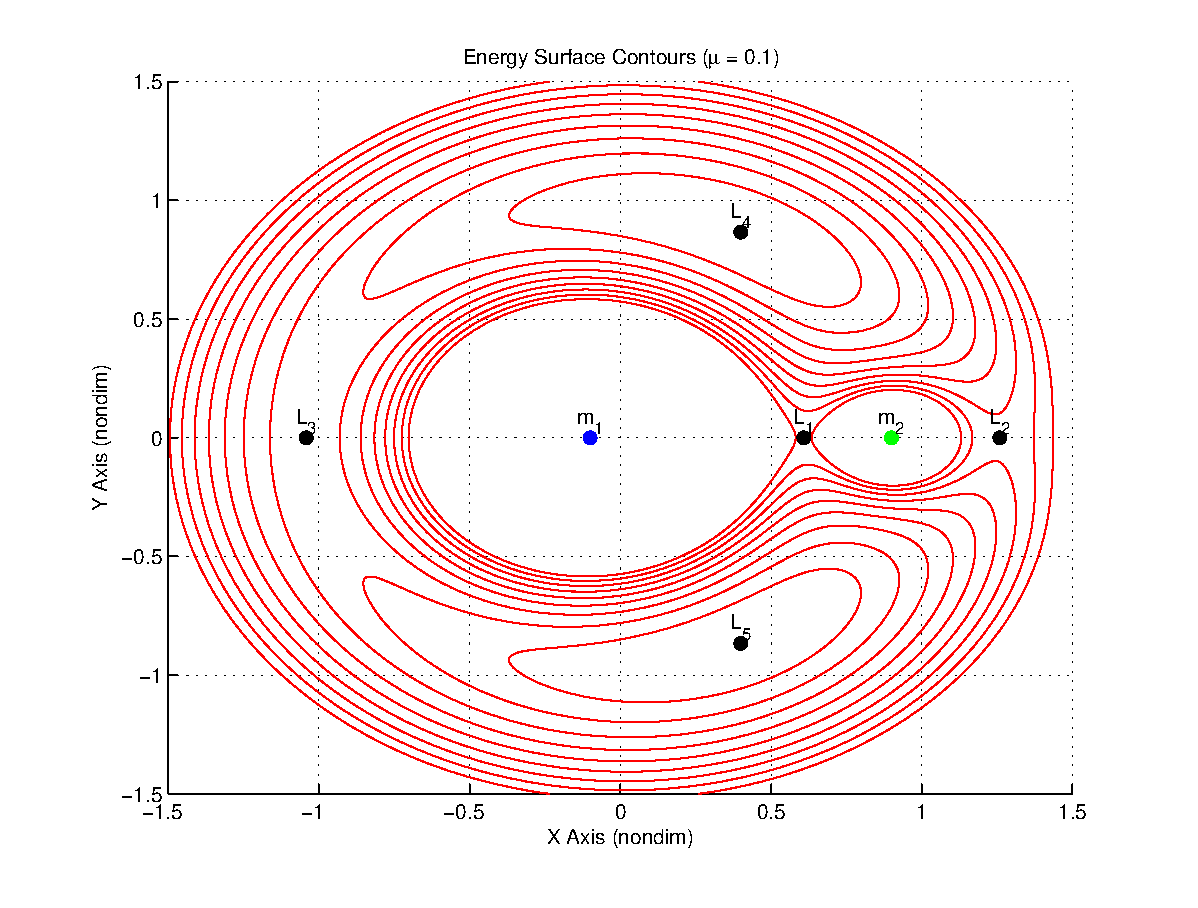
\includegraphics[width=\columnwidth]{energy_contours}
 \end{itemize}
 \end{column}
 \begin{column}{0.5\textwidth}
 \begin{itemize}
 	\item Jacobi energy integral defines a 3D surface of constant energy
 	  \begin{equation*}
		E\left( \bar{r} , \bar{v} \right) = \frac{1}{2}\left( \dot{x}^2 + \dot{y}^2\right) - U\left(x,y \right)
	\label{eq:jacobi}
	\end{equation*}
	\item Contours of constant \( E\) define zero velocity curves and regions of allowable motion
	\end{itemize}
 \end{column}
 \end{columns}
\end{frame}   %-----------------------------%
